\documentclass[aspectratio=1610]{beamer}
\usetheme[sectionpage=progressbar, progressbar=foot]{metropolis} 
\usefonttheme{professionalfonts}   % required for mathspec
\usepackage{mathspec}
\usepackage{bm}
\usepackage{color}
\usepackage{algorithm}
\usepackage{algorithmic}
\usepackage{float}

% ALGORITHMIC
\renewcommand{\algorithmicrequire}{\textbf{Input:}}
\renewcommand{\algorithmicensure}{\textbf{Output:}}

% THEME COLORS REDEF.
\definecolor{Magenta}{HTML}{B50B1E}
\definecolor{deBlue}{HTML}{0E2646}
\setbeamercolor{alerted text}{fg=Magenta}
\setbeamercolor{frametitle}{bg=deBlue}

% ENUM ITEM
\usepackage{fontawesome}
\usepackage{enumitem}
\setitemize{label=\usebeamerfont*{itemize item}%
\usebeamercolor[fg]{itemize item}
\usebeamertemplate{itemize item}}
%\SetLabelAlign{center}{\strut\smash{\parbox[t]\labelwidth{\centering#1}}}
\definecolor{ProGreen}{RGB}{56,146,94}
\definecolor{ConRed}{RGB}{209,28,22}
\newcommand*\pro{%
  \item[\color{ProGreen}\scalebox{1.5}{\faThumbsOUp}]}
\newcommand*\con{%
  \item[\color{ConRed}\scalebox{1.5}{\faThumbsODown}]}

% FONT
%\setsansfont[BoldFont={Fira Sans},
%Numbers={OldStyle}]{Fira Sans Light}
%\setmathsfont(Digits)[Numbers={Lining, Proportional}]{FiraSans Light}

% BIBLIO 
\usepackage[backend=bibtex,style=authoryear-icomp,maxbibnames=9,maxcitenames=2]{biblatex}
\renewcommand*{\nameyeardelim}{\addcomma\addspace}
\bibliography{3DRegistration.bib}
%\setbeamertemplate{bibliography item}{\insertbiblabel} %Removes icon in bibliography 
\renewcommand*{\cite}{\parencite}


% INTRO
\title{3D Rigid Registration}
\subtitle{Algorithms survey}
% \date{\today}
\author{Pasquale Antonante}
%\institute{United Technology Research Center}
%\titlegraphic{\hfill
\includegraphics[height=0.8cm]{imgs/logo_utrc.png}}

%% UTILITIES
\newcommand{\norm}[1]{\left\lVert#1\right\rVert}
\newcommand{\Ealign}{\bm{q}_i-\bm{T}\bm{p}_i}
\DeclareMathOperator*{\argmin}{argmin}
\DeclareMathOperator*{\argmax}{argmax}

\begin{document}
\maketitle

% ===== BEGIN =====

%%%%%%%%%%%%%%%%%%%%%%%%%%%%%%%%%%%%%%%%%%%%%%%%%%%%%%%%%%%
%       Introduction                                      %
%%%%%%%%%%%%%%%%%%%%%%%%%%%%%%%%%%%%%%%%%%%%%%%%%%%%%%%%%%%
\section{Introduction}
%%
\begin{frame}[fragile]{Problem definition}
  \begin{alertblock}{Surface registration}
  Surface registration \textbf{transforms} multiple sets of 3D data points into the same coordinate system so as to \textbf{align overlapping} components of these sets.
\end{alertblock}
\end{frame}

%%
\begin{frame}[allowframebreaks]{Basic notation}
Let's consider two point sets $\bm{P}$ and $\bm{Q}$ we want to find a rigid transformation $\bm{T}$ (rotation $\bm{R}$ and translation $\bm{t}$) that aligns $\bm{Q}$ to $\bm{P}$. 

In general we want to minimize the error $E(\bm{T})$ 
\[ 
%E(\bm{T})=\sum_i{\norm{q_i-\bm{T}p_i}}+E_{\text{reg}}, \quad \text{where}~
E(\bm{T})=E_{\text{align}}+E_{\text{reg}}, \quad \text{where}
\bm{T} = \begin{bmatrix}
   \bm{R} & \bm{t} \\
   \bm{0}^{T} & 1   
\end{bmatrix} 
\]
$E_{\text{align}}$ measure the \textbf{alignment error} while $E_{\text{reg}}$ is a \textbf{regularization} term. 

\framebreak

There are two main metrics to measure the $E_{\text{align}}$
%\begin{equation}
\begin{align}
E_\text{pt-to-pt} &= \sum_i{\norm{\Ealign}^2} \label{pt2pt} \\
E_\text{pt-to-plane} & = \sum_i{\big((\Ealign)\cdot\bm{n}_{q_i}\big)^2} \label{pt2pl}
\end{align}
%\end{equation}

\framebreak

\begin{figure}[htbp]
\begin{center}
\begin{minipage}[b]{0.45\linewidth}
  \centering
  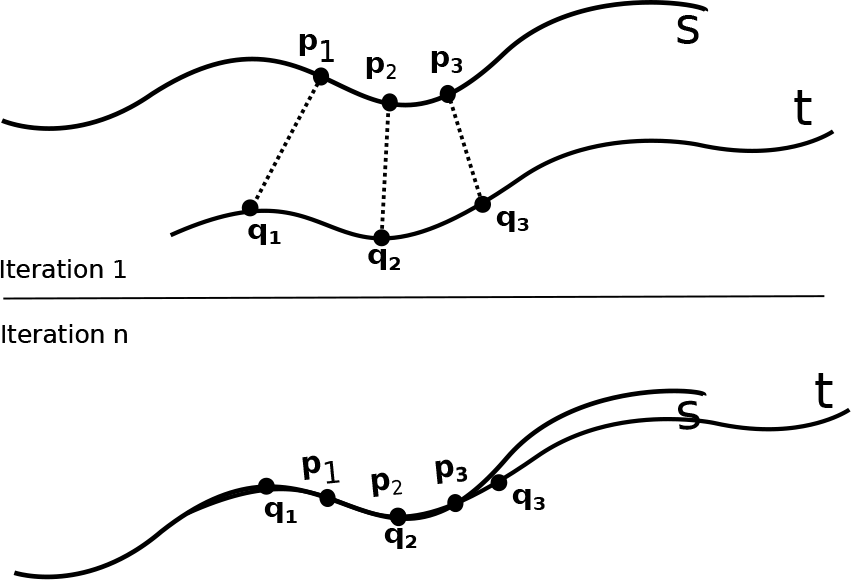
\includegraphics[width=\textwidth,keepaspectratio]{imgs/pt2pt.png}
  \caption{Point-to-Point Distance}
  \label{fig:pt2pt}
\end{minipage}
\begin{minipage}[b]{0.45\linewidth}
  \centering
  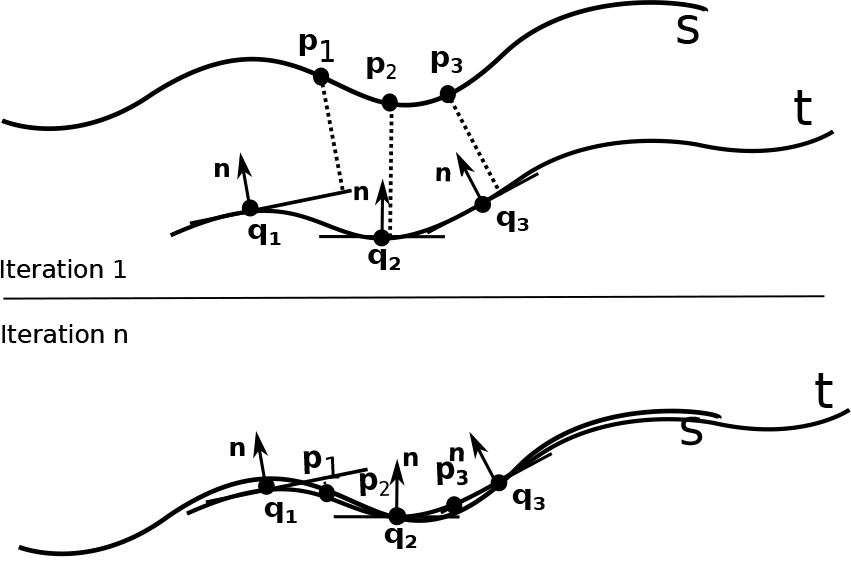
\includegraphics[width=\textwidth,keepaspectratio]{imgs/pt2plane.png}
  \caption{Point-to-Plane Distance}
  \label{fig:pt2pl}
\end{minipage}
\end{center}
\caption{Error metrics \cite{bellekens2014survey}}
\end{figure}

\framebreak

Point-to-plane proved to be more stable and faster to converge but\ldots\textbf{Least Sum of Square Errors} has a closed-form solution!

If we know the \textbf{perfect correspondence} of a subset of points (at least 3) we can compute the rigid transformation
\begin{itemize}
  \item Rotation matrix, e.g. \cite{schonemann1966generalized}, \cite{arun1987least}, \cite{horn1988closed}, \cite{umeyama1991least}
  \item Quaternions, e.g. \cite{horn1987closed}
\end{itemize}

But \textbf{true correspondences} are difficult do be found.
\end{frame}

\begin{frame}[allowframebreaks]{(Non)-Convexity Analysis}
Let's focus on the \textbf{point-to-point} formulation.

Define 
\begin{itemize}
\item Transformation function as $T_x(\alpha)$ that \textbf{affinely transforms} a point $x$, according to some parameter $\alpha=(\bm{R},\bm{t})$
\item The \textbf{distance-to-a-set operator} $d(x)=\inf_{y\in\mathcal{Y}}\norm{x-y}$
\end{itemize}

The \textbf{residual function} $E(\alpha)=d(T_x(\alpha))$ is \emph{convex} if
\begin{itemize}
  \item \emph{(Condition 1)}. Domain $D_{\alpha}$ is a convex set
  \item \emph{(Condition 2)}. The set $\mathcal{Y}$ is convex\footnote{Proof in~\cite{olsson2009branch}}
\end{itemize}

\framebreak

In our case
\begin{itemize}
  \item \emph{Condition 1} cannot be fulfilled for registration with rotation (due to the constraint $\bm{R}\bm{R}^T=\bm{I}$)
  \item \emph{Condition 2} is rarely fulfilled because set $\mathcal{Y}$  is a scan of complex surfaces
\end{itemize}
Therefore, $E(\alpha)$ is \textbf{non-convex}.
\end{frame}

%\begin{frame}{Closed-Form Solution}

%\end{frame}

\begin{frame}{Global vs Local}
\begin{alertblock}{Global vs. Local}
3D Rigid Registration can be classified according to the used \textbf{underlying optimization method}~\cite{rusu2009fast}:
\begin{itemize}
\item \textbf{Global}% (e.g. Genetic Algorithms)
\item \textbf{Local} (e.g. Iterative Closest Point (ICP))
\end{itemize}
\end{alertblock}
\end{frame}

%%%%%%%%%%%%%%%%%%%%%%%%%%%%%%%%%%%%%%%%%%%%%%%%%%%%%%%%%%%
%       Iterative Closest Points                          %
%%%%%%%%%%%%%%%%%%%%%%%%%%%%%%%%%%%%%%%%%%%%%%%%%%%%%%%%%%%
\section{Iterative Closest Points (ICP)} %[Besl & McKay 92]
\begin{frame}[shrink=10]{Basic ICP}
\begin{algorithm}[H]
\begin{algorithmic}[1]
%\STATE Estimate initial registration states
%\STATE Apply initial registration
%\WHILE{Alignment MSE greater than threshold}
%\STATE Compute closest points
%\STATE Compute registration $T$
%\STATE Apply registration
%\ENDWHILE
\REQUIRE $\bm{P}$, $\bm{Q}$ and initial estimation $\bm{T}_0$
\ENSURE $\bm{T}$
\STATE $\bm{T}\gets\bm{T}_0$
\WHILE{not converged}
  \FOR{$i\gets 1$ \TO $N$}
    \STATE $\bm{m}_i\gets\text{FindClosestPointInQ}(\bm{T}\bm{p}_i$)
    \IF{$\norm{\bm{m}_i-\bm{T}\bm{p_i}}\leq d_{\text{max}}$}
      \STATE $\omega_i\gets 1$
    \ELSE
      \STATE $\omega_i\gets 0$
    \ENDIF
  \ENDFOR
  \STATE $\bm{T}\gets\argmin\limits_T \sum\limits_i \omega_i \norm{\bm{m}_i-\bm{T}\bm{p}_i}$
\ENDWHILE
\end{algorithmic}
\caption{Iterative Closest Points (ICP)}
\label{alg:ICP}
\end{algorithm}
\end{frame}

\begin{frame}{Considerations}
\begin{itemize}[wide, labelsep=2em]
  \pro Solves the correspondence problem
  \con May get caught in local minima
  \con Require (and depends) an initial registration guess
  \con Computes closest points set each iteration
\end{itemize}
\end{frame}

\begin{frame}{Local Optimization Method}
%ICP is a \textbf{local optimization algorithm} and may get caught in local minima.

There is a lot of work around ICP addressing the local minima issue, some relevant methods are:
\begin{itemize}
	\item \textbf{Robustified Local Methods}
	\item \textbf{Global Methods} (GA, Particle filtering, Simulated Annealing)
	\item \textbf{Globally Optimal Methods} (i.e. BnB)
\end{itemize}
\end{frame}



%%%%%%%%%%%%%%%%%%%%%%%%%%%%%%%%%%%%%%%%%%%%%%%%%%%%%%%%%%%
%       Global Go-ICP                                     %
%%%%%%%%%%%%%%%%%%%%%%%%%%%%%%%%%%%%%%%%%%%%%%%%%%%%%%%%%%%
\section{GO-ICP (2016)}
%%
\begin{frame}{Introduction}
Global-ICP (GO-ICP)~\cite{goicp} optimally solves 3D registration by mixing ICP and BnB.
\begin{figure}[htbp]
\begin{center}
  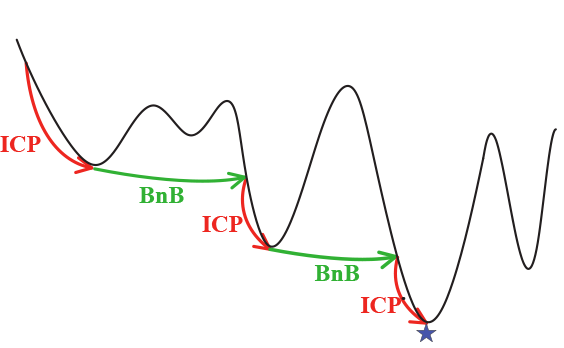
\includegraphics[width=\textwidth,height=0.45\textheight,keepaspectratio]{imgs/GOICP_collaboration.png}
  \caption{Collaboration of BnB and ICP.}
  \label{fig:goicp_collaboration}
\end{center}
\end{figure}
\end{frame}

\begin{frame}[allowframebreaks]{Domain Parametrization}
To parametrize the search space let's consider the \textbf{angle-axis} representation of rotations, obtaining
\begin{itemize}
	\item the rotation space $SO(3)$ is parametrized in a solid radius-$\pi$ ball 
	\item the translation is assumed to be within the cube $[-\xi,\xi]^3$ (denoted as $C_t$)
\end{itemize}
\begin{figure}[htbp]
\begin{center}
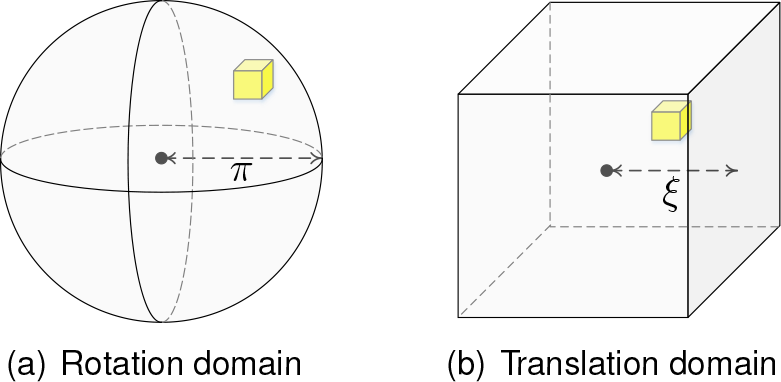
\includegraphics[width=\textwidth,height=0.3\textheight,keepaspectratio]{imgs/GOICP_parametrization.png}
\caption{$SE(3)$ space parametrization in GO-ICP}
\label{default}
\end{center}
\end{figure}
\end{frame}

%%
\begin{frame}[allowframebreaks]{Bounding Functions}
For ease of manipulation, let's use the minimum cube $[−\pi,\pi]^3$ that encloses the $\pi$-ball centered in $\bm{r}_0$ as $C_r$.

\begin{theorem}[Uncertainty radius]
Given a 3D point $\bm{p}$, a rotation cube $C_r$ of half side-length $\sigma_r$ with $r_0$ as the center and examining the maximum distance from $\bm{R}_{\bm{r}}\bm{p}$ to $\bm{R}_{\bm{r_0}}\bm{p}$, we have $\forall\bm{r}\in C_r$,
\[ \norm{\bm{R}_r\bm{p}-\bm{R}_{r_0}\bm{p}} \leq 2\sin(\min(\sqrt{3}\sigma_r/2,\pi/2))\norm{\bm{p}} = \gamma_r \]
Or similarly, given a translation cube $C_t$ with half side-length $\sigma_t$ centered at $\bm{t_0}$, we have $\forall\bm{t}\in C_t$
\[ \norm{(\bm{p}+\bm{t}) - (\bm{p}-\bm{t}_0)} \leq \sqrt{3}\sigma_t = \gamma_t \]
\end{theorem}
\end{frame}

%%
\begin{frame}{BnB Bounds}
%Instead of direct 6D space exploration, a \textbf{nested BnB} search is proposed:
%\begin{itemize}
%  \item \textbf{Outer BnB} searches the rotation space of $SO(3)$
%  \item \textbf{Inner BnB} called by the outer BnB, solves the translation problem
%\end{itemize}

%The upper $\overline{E}$ bound and the lower bound $\underline{E}$ for both BnB can be derived~\cite{goicp}. 

%\framebreak
For a given rotation cube $C_r$
\begin{equation}
  \begin{array}{ll} 
  \overline{E}_r &= \min\limits_{\forall\bm{t}\in\mathcal{C}_t} \sum\limits_i e_i (\bm{R}_{\bm{r}_0}, \bm{t})^2 \\
  \underline{E}_r &= \min\limits_{\forall\bm{t}\in\mathcal{C}_t} \sum\limits_i \max \big(e_i(\bm{R}_{\bm{r}_0},t)-\gamma_{r_i},0\big)^2
  \end{array}
\end{equation}
Similarly, for a given translation cube $C_t$
\begin{equation}
\begin{array}{ll}
  \overline{E}_t &= \sum\limits_i \max\big( e_i(\bm{R}_{\bm{r}_0},\bm{t_0})-\gamma_{r_i}, 0 \big)^2 \\
  \underline{E}_t &= \sum\limits_i \max \big( e_i(\bm{R}_{\bm{r}_0},\bm{t_0}) - (\gamma_{r_i} + \gamma_t),0 \big)^2
\end{array}
\label{eq:goicp_outerbound}
\end{equation}
where $e_i(\bm{R},\bm{t})=\norm{\bm{q}_{j^*}-\bm{R}\bm{p}_i}$, with $\bm{q}_{j^*}$ denoted as optimal correspondence of $\bm{p}_i$; $\mathcal{C}_r$ and $\mathcal{C}_t$ are the initial cubes.
\end{frame}

%%
\begin{frame}[shrink=36]{Go-ICP algorithm}
\begin{columns}
\begin{column}{0.5\textwidth}
  \begin{algorithm}[H] %% outer
  \begin{algorithmic}[1]
  \REQUIRE $\bm{P}$, $\bm{Q}$, threshold $\epsilon$, initial cubes $\mathcal{C}_r$, $\mathcal{C}_t$
  \ENSURE Globally minimal error $E^*$ and corresponding $\bm{r}^*$, $\bm{t}^*$
  \STATE Put $\mathcal{C}_r$ into priority queue $Q_r$
  \STATE Set $E^*=+\infty$
  \LOOP
    \STATE Read out a cube with lowest $\underline{E}_r$ from $Q_r$
    \STATE Quit if $E^*-\underline{E}_r<\epsilon$
    \STATE Divide the cube into 8 sub-cubes
    \FORALL{sub-cube $C_r$}
      \STATE Compute $\overline{E}_r$ for $C_r$ and corresponding optimal $\bm{t}$ by calling alg.\ref{alg:goicp_inner} with $\bm{r}_0$, $\gamma_r=0$ and $E^*$
      \IF{$\overline{E}_r<E^*$}
        \STATE Run ICP with initialization $(\bm{r}_0,\bm{t})$
        \STATE Update $E^*$, $r^*$ and $t^*$ with ICP results
      \ENDIF
      \STATE Compute $\underline{E}_r$ for $C_r$ by calling alg.\ref{alg:goicp_inner} with $\bm{r}_0$, $\gamma_r$ and $E^*$
      \IF{$\underline{E}_r \geq E^*$}
        \STATE Discard $C_r$ and continue the loop
      \ENDIF
      \STATE Put $C_r$ into $Q_r$
    \ENDFOR
  \ENDLOOP
  \end{algorithmic}
  \caption{Go-ICP -- Outer BnB}
  \label{alg:goicp_outer}
  \end{algorithm}
\end{column}

\begin{column}{0.5\textwidth}

  \begin{algorithm}[H] %% inner
  \begin{algorithmic}[1]
  \REQUIRE $\bm{P}$, $\bm{Q}$, threshold $\epsilon$, initial cube $\mathcal{C}_t$, rotation $r_0$, rotation uncertainty radii $\gamma_r$, so-far-best-error $E^*$
  \ENSURE Minimal error $E_t^*$ and corresponding $\bm{t}^*$
  \STATE Put $\mathcal{C}_t$ into priority queue $Q_t$
  \STATE Set $E^*_t = E^*$
  \LOOP
    \STATE Read out a cube with lowest $\underline{E}_t$ from $Q_t$
    \STATE Quit the loop if $E_t^*-\underline{E}_t<\epsilon$
    \STATE Divide the the cube into 8 sub-cubes
    \FORALL{sub-cube $C_T$}
      \STATE Compute $\overline{E}_t$ for $C_t$ by~\ref{eq:goicp_outerbound} with $\bm{r}_0$, $\bm{t}_0$ and $\gamma_r$
      \IF{$\overline{E}_t<E_t^*$}
        \STATE Update $E_t^*=\overline{E}_t$, $t^*=t_0$
      \ENDIF
      \STATE Compute $\underline{E}_t$ for $C_t$ by~\ref{eq:goicp_outerbound} with $\bm{r}_0$, $\bm{T}_0$ and $\gamma_t$
      \IF{$\underline{E}_t \geq E_t^*$}
        \STATE Discard $C_t$ and continue the loop
      \ENDIF
      \STATE Put $C_t$ into $Q_r$
    \ENDFOR
  \ENDLOOP
  \end{algorithmic}
  \caption{Go-ICP -- Inner BnB}
  \label{alg:goicp_inner}
  \end{algorithm}

\end{column}
\end{columns}
\end{frame}

%%
\begin{frame}[allowframebreaks]{Experiment}
\begin{figure}[htbp]
\begin{center}
  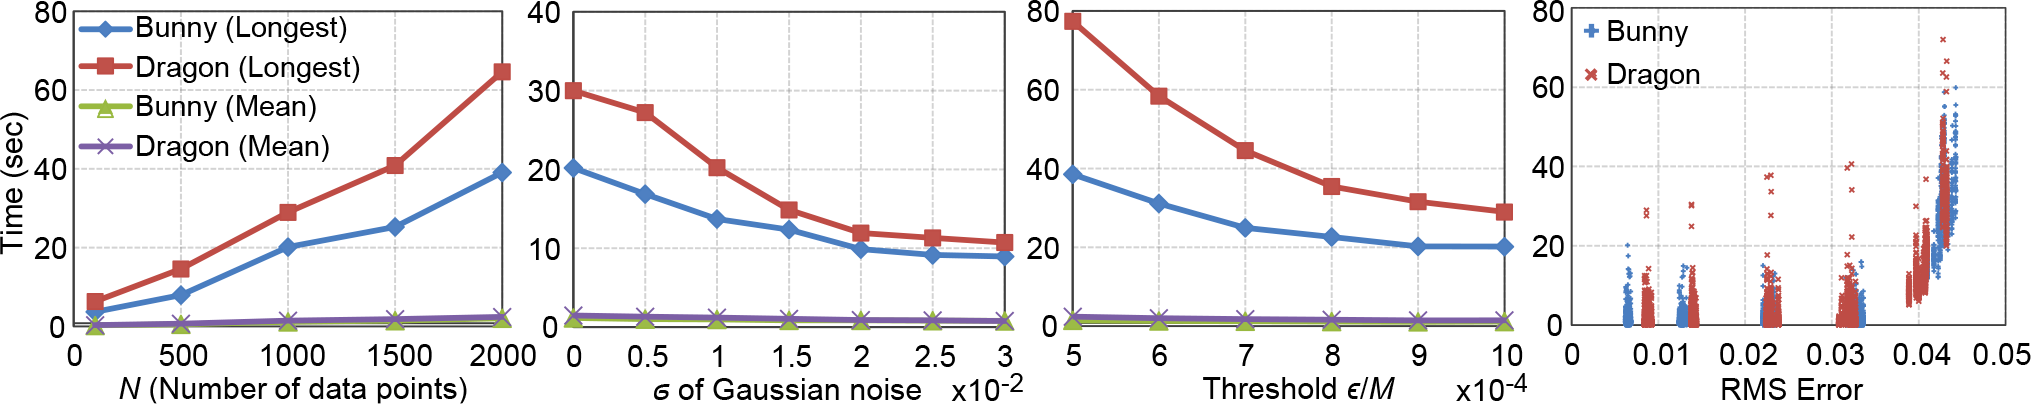
\includegraphics[width=\textwidth,height=0.5\textheight,keepaspectratio]{imgs/GOICP_eval.png}
  \caption{Running time of the Go-ICP method on the bunny and dragon point-sets with respect to different factors.}
  \label{fig:goicp_evaluation}
\end{center}
\end{figure}
\hspace{2em}
\begin{figure}[htbp]
\begin{center}
  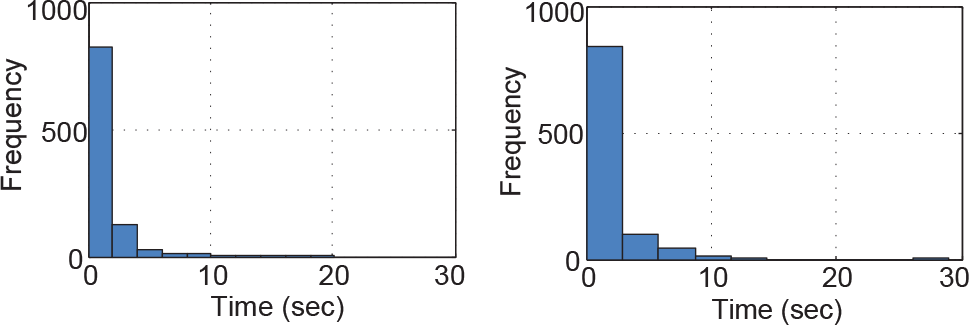
\includegraphics[width=\textwidth,height=0.5\textheight,keepaspectratio]{imgs/GOICP_timehistogram.png}
  \caption{Running time histograms of Go-ICP for the bunny (left) and dragon (right) point-sets.}
  \label{fig:goicp_timehistogram}
\end{center}
\end{figure}
\end{frame}

%%
\begin{frame}{Go-ICP Trimming}
In \cite{goicp} a \textbf{trimmed} version of the algorithm is also proposed. Specifically, in each iteration, only a subset $\bm{S}$ of the data points are used for motion computation.

This is a strategy to obtain a more robust statistic by excluding some of the extreme values.
\end{frame}

\begin{frame}{Considerations}
\begin{itemize}[wide, labelsep=2em]
  \pro Finds the global optimal solution
  \pro Defines upper and lower bound in domain regions
  \pro Not constrained to ICP variants
  \pro Parallelism can speed up computation a lot
  \con Limited to pt-to-pt distance
  \con Computes closest points set each iteration
  \con Computationally demanding
\end{itemize}
\end{frame}

%%%%%%%%%%%%%%%%%%%%%%%%%%%%%%%%%%%%%%%%%%%%%%%%%%%%%%%%%%%
%       Generalized ICP                                   %
%%%%%%%%%%%%%%%%%%%%%%%%%%%%%%%%%%%%%%%%%%%%%%%%%%%%%%%%%%%
\section{Generalized ICP (2009)}
%%
\begin{frame}[allowframebreaks]{Derivation}
The Generalized-ICP~\cite{gicp} uses \textbf{probabilistic approach} to increase robustness by changing
\[ \bm{T}\gets\argmin\limits_T \sum\limits_i \omega_i \norm{\bm{m}_i-\bm{T}\bm{p}_i} \]
in the basic ICP algorithm (alg.~\ref{alg:ICP}).

\framebreak

For the purpose of this section let's assume that:
\begin{itemize}
  \item $\bm{p}_i$ is a correspondence for $\bm{q}_i$ (and vice versa) - W.L.O.G.
  \item $\hat{\bm{P}}=\{\hat{\bm{p}}_i\}, \quad \bm{p}_i \sim \mathcal{N}(\hat{\bm{p}}_i,\bm{C}_i^P)$
  \item $\hat{\bm{Q}}=\{\hat{\bm{q}}_i\}, \quad \bm{q}_i \sim \mathcal{N}(\hat{\bm{q}}_i,\bm{C}_i^Q)$
\end{itemize}
where $\bm{C}_i^P$ and $\bm{C}_i^Q$ are covariance matrices associated with the measured points.

%\framebreak
%%(geometrically consistent with no errors due to occlusion or sampling)
%Assuming \textbf{perfect correspondences} we have a transformation $\bm{T}^*$ such that
%\[\hat{\bm{q}_i}=\bm{T}^*\hat{\bm{p}_i} \]

%For an arbitrary rigid transformation, $\bm{T}$, define
%\[ d_i^{(\bm{T})}=\bm{q}_i-\bm{T}\bm{p}_i \]

%Consider the distribution from which $d(\bm{T}^*)$ is drawn. Since $\bm{p}_i$ and $\bm{q}_i$ are assumed to be drawn from independent Gaussians,
%\[ 
%\begin{array}{ll}
%d_i^{(\bm{T}^*)} &\sim \mathcal{N}\Big(\bm{q}_i - (\bm{T}^*)\bm{p}_i,~ \bm{C}_i^Q +(\bm{T}^*)\bm{C}_i^P(\bm{T}^*)^T \Big) \\
%&= \mathcal{N}\Big( 0,~ \bm{C}_i^Q +(\bm{T}^*)\bm{C}_i^P(\bm{T}^*)^T \Big)
%\end{array}
%\]

\framebreak

%We can use \textbf{Maximum likelihood estimation} to iteratively compute $\bm{T}$
%\[ \bm{T} = \argmax\limits_{\bm{T}} \prod\limits_i p\big( d_i^{(\bm{T})} \big)
%     = \argmax\limits_{\bm{T}} \sum\limits_i \log \big(
%     p\big( d_i^{(\bm{T})} \big) \big)
%\]
%that can be simplified to
%\begin{equation}
%\bm{T} = \argmin\limits_{\bm{T}} \sum\limits_i {d_i^{(\bm{T})}}^T ( \bm{C}_i^Q+ \bm{T} \bm{C}_i^P \bm{T}^T)^{-1} d_i^{(\bm{T})}
%\end{equation}
%This defines the \textbf{key step} of the Generalized-ICP algorithm.


We can use \textbf{Maximum likelihood estimation} to iteratively compute $\bm{T}$
\[ \bm{T} = \argmax\limits_{\bm{T}} \prod\limits_i p\big( \Ealign \big)
     = \argmax\limits_{\bm{T}} \sum\limits_i \log \big(
     p\big( \Ealign \big) \big)
\]
that can be simplified to
\begin{equation}
\bm{T} = \argmin\limits_{\bm{T}} \sum\limits_i (\Ealign)^T ( \bm{C}_i^Q+ \bm{T} \bm{C}_i^P \bm{T}^T)^{-1} (\Ealign)
\end{equation}
This defines the \textbf{key step} of the Generalized-ICP algorithm (Mahalanobis distance).
\end{frame}

\begin{frame}{Results}
\begin{figure}[htbp]
\begin{center}
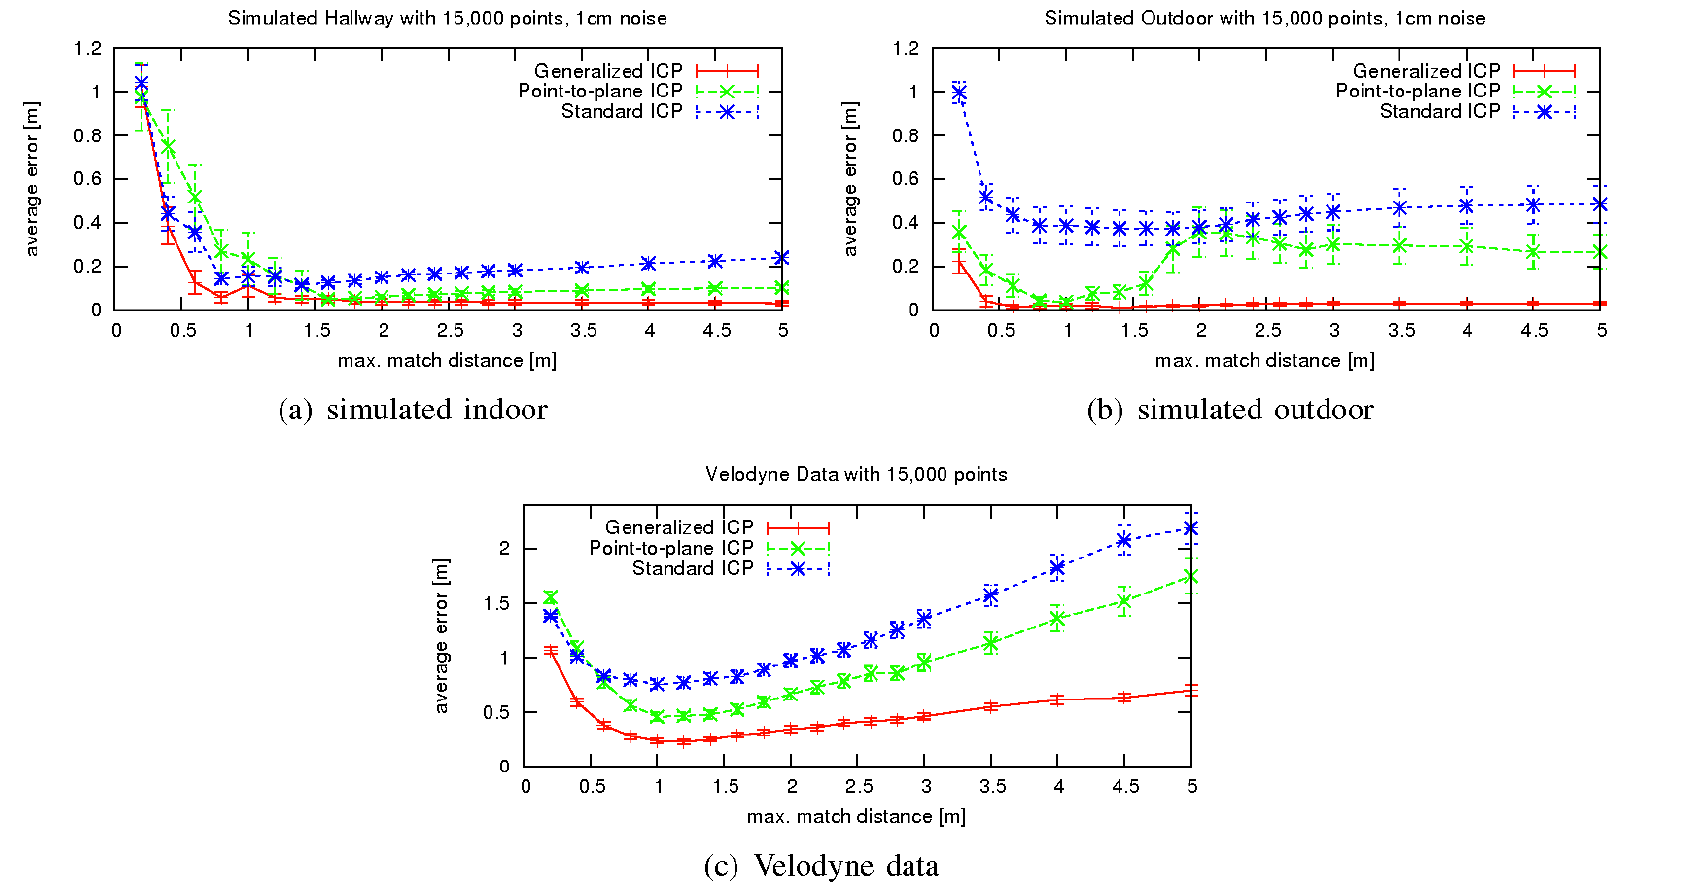
\includegraphics[width=\textwidth,keepaspectratio]{imgs/gicp.png}
\caption{Average error}
\label{fig:gicp}
\end{center}
\end{figure}
\end{frame}

\begin{frame}{Considerations}
\begin{itemize}[wide, labelsep=2em]
  \pro Probabilistic approach
  \pro Covariance matrices give good flexibility
  \con Covariance matrices can be complex to compute
  \con Might get caught in local minima
  \con Still dependent on initial guess
  \con No closed form solution for $\bm{T}$ is available
\end{itemize}
\end{frame}

%%%%%%%%%%%%%%%%%%%%%%%%%%%%%%%%%%%%%%%%%%%%%%%%%%%%%%%%%%%
%       Learning Anisotropic ICP                          %
%%%%%%%%%%%%%%%%%%%%%%%%%%%%%%%%%%%%%%%%%%%%%%%%%%%%%%%%%%%
\section{Learning Anisotropic ICP (2016)}

\begin{frame}{Principle}
%Within the generalized ICP framework, we need to have some strategies to determine the values of covariances.

\begin{figure}[htbp]
\begin{center}
  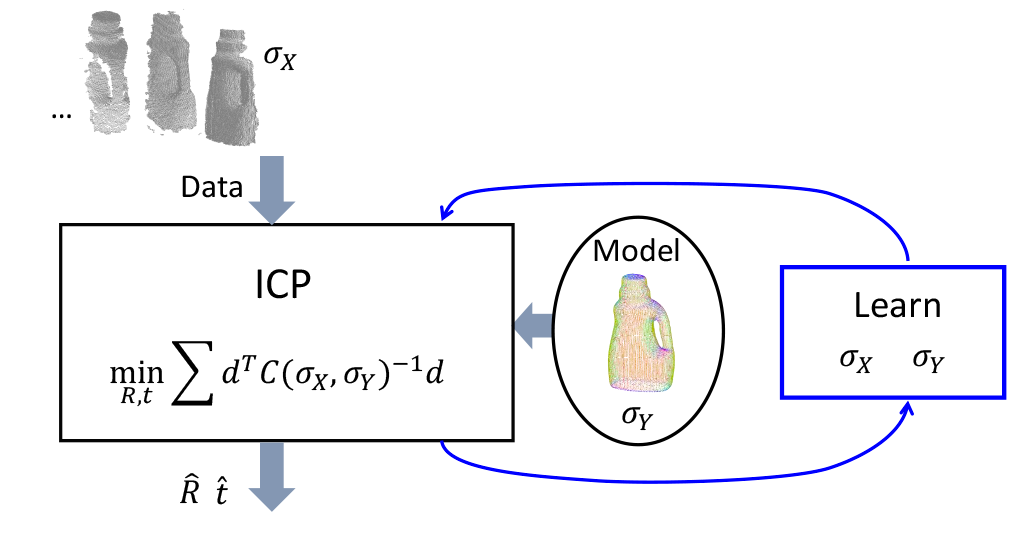
\includegraphics[height=0.5\textheight,keepaspectratio]{imgs/LAICP.png}
  %\caption{LA-ICP}
  \label{fig:LAICP}
\end{center}
\end{figure}
\textbf{Idea:} Learning Anisotropic ICP \cite{lee2016learning}, assumes anisotropic Gaussian, and estimates the covariance. The learning scheme does not require manual tuning and the covariance is continually updated from observed data.
\end{frame}


\begin{frame}{Pros and Cons}
\begin{itemize}[wide, labelsep=2em]
\setlength\itemsep{1em}
\pro Assumes anisotropic noise
\pro Reduces computational overhead due to covariance matrices
\con Still local optimization method
\end{itemize}
\end{frame}

%%%%%%%%%%%%%%%%%%%%%%%%%%%%%%%%%%%%%%%%%%%%%%%%%%%%%%%%%%%
%       Fast Global Registration                          %
%%%%%%%%%%%%%%%%%%%%%%%%%%%%%%%%%%%%%%%%%%%%%%%%%%%%%%%%%%%
\section{Fast Global Registration (2016)}
%%
\begin{frame}{Introduction}
Let $\mathcal{K}=\{(p,q)\}$ be a set of \textbf{correspondences} collected by matching points from $\bm{P}$ and $\bm{Q}$.% as described in slide \ref{fpfh_correspondences}.

We want to minimize:
\begin{equation}
\label{eq:fastgo_obj}
E(\bm{T})=\sum_{(p,q)\in\mathcal{K}}\rho({\norm{q_i-\bm{T}p_i}})
\end{equation}
where $\rho(\cdot)$ is a \textbf{robust penalty function}, i.e. \alert{scaled Geman-McClure estimator}.
\end{frame}

%%
\begin{frame}{Scaled Geman-McClure estimator}
Using this estimator small residuals are penalized in the LS sense:
\begin{equation}
\rho(x)=\frac{\mu x^2}{\mu+x^2}
\end{equation}
\begin{figure}[htbp]
\begin{center}
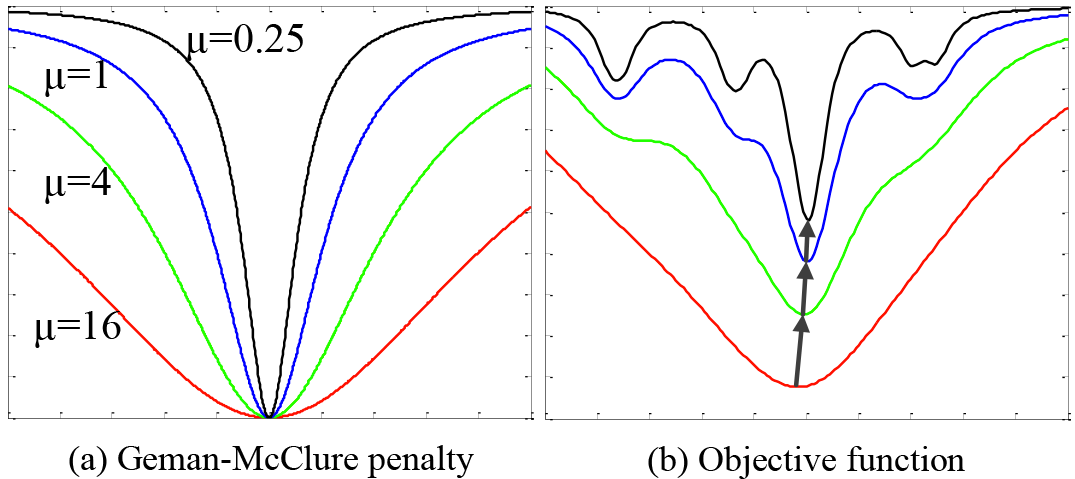
\includegraphics[width=\textwidth,height=0.5\textheight,keepaspectratio]{imgs/geman_estimator.png}
\caption{Geman-McClure estimator vs. Objective function (\ref{eq:fastgo_obj})}
\label{fig:geman}
\end{center}
\end{figure}
%The parameter $\mu$ controls the range within which residuals have a significant effect on the objective.
\end{frame}

%%
\begin{frame}[allowframebreaks]{Black-Ragarajan duality}
Objective function (\ref{eq:fastgo_obj}) is difficult to optimize directly, so the authors used \textbf{Black-Ragarajan duality} between line process and robust estimation \cite{black1996unification}.

Let's $\mathbb{L}=\{l_{(p,q)}\}$ a line process over the correspondences, we can write a new objective function optimized over $\bm{T}$ and $\mathbb{L}$.
\begin{equation}
\label{eq:fastgo_fullobj}
E(\bm{T},\mathbb{L})=\sum_{(p,q)\in\mathcal{K}}\big(l_{(p,q)}\norm{p-\bm{T}q}^2+\Psi(l_{(p,q)})\big)
\end{equation}
where  
\[ \Psi(l_{(p,q)}) = \mu \big( \sqrt{l_{(p,q)}} -1 \big)^2 \]

Minimizing (\ref{eq:fastgo_fullobj}) over $\mathbb{L}$ we have:
\[ \frac{\partial{E}}{\partial{l_{(p,q)}}} = \norm{p-\bm{T}q} +\mu\frac{\sqrt{l_{(p,q)}} -1}{\sqrt{l_{(p,q)}}}  = 0 \]
Solving for $l_{(p,q)}$ yields
\begin{equation}\label{eq:fgr_lattice}
 l_{(p,q)} =  \Bigg( \frac{\mu}{\mu + \norm{p-\bm{T}q}^2}  \Bigg)^2
 \end{equation}

Substituting $l_{(p,q)}$ in (\ref{eq:fastgo_fullobj}) we obtain (\ref{eq:fastgo_obj}). Thus \textbf{optimizing objective (\ref{eq:fastgo_fullobj}) yields a solution $\bm{T}$ that is also optimal for the original objective (\ref{eq:fastgo_obj})}.

\alert{What about the correspondences?}
\end{frame}

%%

\begin{frame}[allowframebreaks]{Fast Point Feature Histogram (FPFH)}
\begin{itemize}
\item The goal of FPFH is to encode a point's \textbf{k-neighborhood geometrical properties}.
\item The complexity is $O(kN)$, where $k$ is the number of neighbors for each point~\cite{rusu2009fast}
\item It is based on the \textbf{Simple Point Feature Histogram (SPFH)}
\end{itemize}

\framebreak

\textbf{Simple Point Feature Histogram (SPFH)}
\par
For each query point $\bm{p}_q$, 
\begin{itemize}
\item Compute the $k$-neighborhood set $P_k^q$
\item Compute the tuple $(\alpha,\phi,\theta)$ between $\bm{p}_q$ and each $\bm{p}_k\in P_k^q$
\begin{equation}
\begin{array}{ll}
\bm{u} & = \bm{n}_q \\
\bm{v} & = \bm{u} \times \frac{(\bm{p}_k-\bm{p}_q)}{\norm{\bm{p}_k-\bm{p}_q}} \\
\bm{w} & = \bm{u} \times \bm{v}
\end{array}	\qquad \Rightarrow \qquad
\begin{array}{ll}
\alpha & = \bm{v}\cdot\bm{n}_k \\
\phi & = \bm{u} \cdot \frac{(\bm{p}_k-\bm{p}_q)}{\norm{\bm{p}_k-\bm{p}_q}_2} \\
\theta & = \arctan(\bm{w}\cdot\bm{n}_q, \bm{u}\cdot\bm{n}_k)
\end{array}
\end{equation}
\item Bin all $(\alpha,\phi,\theta)$ into a histogram
\end{itemize}

\framebreak

To compute the FPFH histogram feature:
\begin{itemize}
  \item for each query point $\bm{p}_q$ compute the SPFH
  \item for each point its $k$ neighbors are re-determined, and the neighboring SPFH values are used to weight the final histogram of $\bm{p}_q$ (called FPFH) as in eq.\ref{eq:fpfh}
\end{itemize}

\begin{equation}
\label{eq:fpfh}
\text{FPFH}(\bm{p}_q)=\text{SPFH}(\bm{p}_q)+\frac{1}{k}\sum_{i=1}^{k}\frac{1}{\omega_k}\cdot\text{SPFH}(\bm{p}_k)
\end{equation}
where the weight $\omega_k$ represents a distance between the query point $\bm{p}_q$ and a neighbor point $\bm{p}_k$ in some given metric space.

%\begin{figure}[htbp]
%\begin{center}
%\begin{minipage}[b]{0.45\linewidth}
%            \centering
%            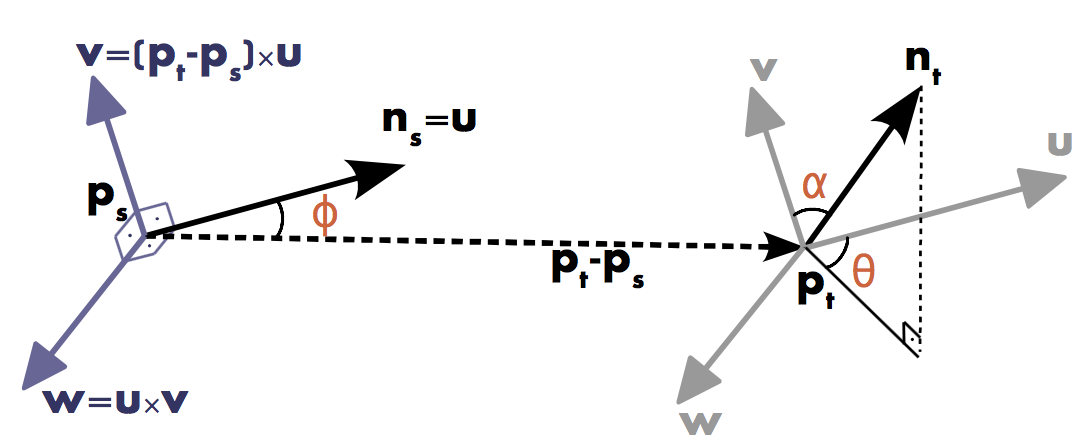
\includegraphics[width=\textwidth,height=0.5\textheight,keepaspectratio]{imgs/DarbouxFrame.png}
%	    \caption{Darboux Frame}
%            \label{fig:DarbouxFrame}
%        \end{minipage}
%        \hspace{0.5cm}
%        \begin{minipage}[b]{0.45\linewidth}
%            \centering
%             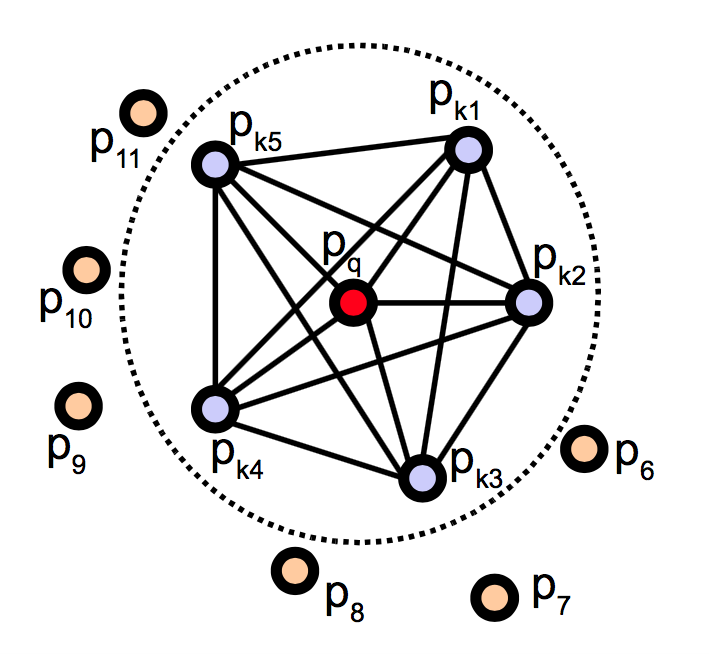
\includegraphics[width=\textwidth,height=0.3\textheight,keepaspectratio]{imgs/FPFH_NN.png}
%	    \caption{The influence region diagram for a Point Feature Histogram.}
%            \label{fig:FPFH_NN}
%        \end{minipage}
%\end{center}
%\end{figure}
\end{frame}

%%
\begin{frame}[allowframebreaks]{Correspondences set}\label{fpfh_correspondences}
The correspondence set is build as following, let 
\begin{itemize}
\item $F(\bm{P})=\{F(\bm{p}):\bm{p}\in\bm{P}\}$ the FPFH of points in $\bm{P}$
\item $F(\bm{Q})=\{F(\bm{q}):\bm{q}\in\bm{Q}\}$ the FPFH of points in $\bm{Q}$
\end{itemize}

$\mathcal{K}_1$ is the set containing the nearest neighbor of $F(\bm{p})$ among $F(\bm{Q})$, and vice versa.

\framebreak

We can improve the correspondences set by applying:
\begin{description}
\item[Reciprocity test] A correspondence pair $(\bm{p}, \bm{q})$ is selected from $\mathcal{K}_1$ if and only if $F(\bm{p})$ is the nearest neighbor of $F(\bm{q})$ among $F(\bm{P})$ and $F(\bm{q})$ is the nearest neighbor of $F(\bm{p})$ among $F(\bm{Q})$. The resulting correspondence set is denoted by $\mathcal{K}_2$
\item[Tuple test] Randomly pick 3 correspondence pairs $(\bm{p_1}, \bm{q_1})$, $(\bm{p_2}, \bm{q_2})$, $(\bm{p_3}, \bm{q_3})$ from $\mathcal{K}_2$ and check if the tuples $(\bm{p_1}, \bm{p_2}, \bm{p_3})$ and $(\bm{q_1}, \bm{q_2}, \bm{q_3})$ are compatible
\[ \forall i\neq j, \quad \tau \le \frac{\norm{p_i-p_j}}{\norm{q_i-q_j}} \le \frac{1}{\tau}, \quad \tau=0.9 \]
This is the set used by the algorithm $\mathcal{K} = \mathcal{K}_3$
\end{description}
\end{frame}

%%
\begin{frame}{Fast Global Registration Algorithm}
Let $D$ be the diameter of the largest surface and $\delta$ the distance threshold for genuine correspondence
\begin{algorithm}[H]
\begin{algorithmic}[1]
\STATE{Compute normals $\{\bm{n}_p\}$ and $\{\bm{n}_q\}$}
\STATE{Compute $F(\bm{P})$ and $F(\bm{Q})$}
\STATE{Compute $\mathcal{K}=\mathcal{K}_3$}
%\STATE{Build $\mathcal{K}_1$ by computing nearest neighbors between $\bm{F}(\bm{P})$ and $\bm{F}(\bm{Q})$}
%\STATE{Apply reciprocity test on $\mathcal{K}_1$ to get $\mathcal{K}_2$}
%\STATE{Apply tuple test on $\mathcal{K}_2$ to get $\mathcal{K}_3$}
\STATE{$\bm{T}\gets \bm{I},~\mu\gets D^2$}
\WHILE{not converged or $\mu>\delta^2$}
\FOR{$(p,q)\in\mathcal{K}$}
\STATE{Compute $l_{(p,q)}$ using equation~\ref{eq:fgr_lattice}}
\ENDFOR
\STATE{Compute $\bm{T}$ (closed form~\cite{horn1987closed})}
\STATE{Every four iterations $\mu\gets \mu/2$}
\ENDWHILE
\end{algorithmic}
\caption{Fast Global Registration}
\label{alg:fastglobalregistration}
\end{algorithm}
\end{frame}

%%
\begin{frame}[allowframebreaks]{Performance}
\begin{figure}[htbp]
\begin{center}
\centering
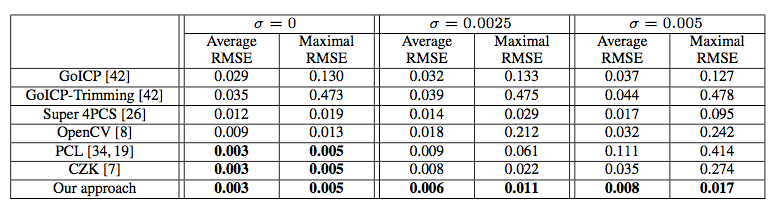
\includegraphics[width=1.5\textheight,keepaspectratio]{imgs/RMSE_fgr.png}
\caption{Average and maximal RMSE achieved by global registration algorithms on synthetic range images with noise level $\sigma$}
\label{fig:fastgo_RMSR}
\end{center}
\end{figure}
\begin{figure}[htbp]
\begin{center}
\centering
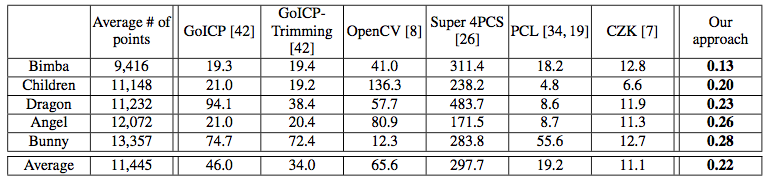
\includegraphics[width=1.5\textheight,keepaspectratio]{imgs/Time_fgr.png}
\caption{Running times of global registration methods, measured in seconds}
\label{fig:fastgo_time}
\end{center}
\end{figure}

%\framebreak

%\begin{figure}[htbp]
%\begin{center}
%\centering
%\includegraphics[width=1.5\textheight,keepaspectratio]{imgs/LocalRMSE_fgr.png}
%\caption{Controlled comparison with local methods. Perturbation refers to initialization}
%\label{fig:fastgo_lacalRMSE} 
%\end{center}
%\end{figure}
\begin{figure}[htbp]
\begin{center}
\centering
\includegraphics[width=1.5\textheight,keepaspectratio]{imgs/LocalTime_fgr.png}
\caption{Timing comparison with local algorithms, measured in seconds}
\label{fig:fastgo_lacalTime}
\end{center}
\end{figure}
\end{frame}

%%
\begin{frame}{Pros and Cons}
\begin{itemize}[wide, labelsep=2em]
\setlength\itemsep{1em}
\pro Global optimization
%\pro Matches ICP performance (both local and global)
\pro One order of magnitude faster
\pro Does not require initialization
\pro Correspondences computed only once but their weight change
\con No proof of global convergence in the paper
\end{itemize}
\end{frame}

% ===== BIB =====

\begin{frame}[allowframebreaks]{References}
\printbibliography
\end{frame}

\end{document}